\documentclass{article}

\usepackage{./settings/preamble}



\begin{document}
\begin{center}
    {\LARGE\color{mBlue} \textbf{Fitting \& Alignment}}\\\vspace*{.1cm}
    S.Sanjith : 190562G
\end{center}
\vspace*{-.5cm}
\HRule
\begin{abstract}
    Despite the advancement in fitting approaches, RANSAC  is a good algorithm that can deal with higher outlier ratios up to 50\%.    In this report, we will talk about the implementation of RANSAC in two different situations. In the first part of the report, we will fit a circle with given points. Then we try to fit two shapes using homographic transformation. In the third part, we will analyze an application of finding homographic transformation between two images. Finally, we will try to generalize the RANSAC approach to find the best circle and suitable homographic transformation used in stitching two images.
\end{abstract}



\section{Fitting Circle}
Any circle can be defined by a minimum of three points. That is a circle is fully defined if it is expected to go through three points. Hence it is not suitable to fit a circle accurately with a given number of points.  By defining the total euclidean distances as the measure of error, a better choice for the circular fit can be achieved. 

 
\subsection*{Randy Bullock}
Two famous approaches for the fitting circle are circular regression and randy bullock fit. With few implementations, it is observed that the randy bullock fit is doing better in the noisy environment. \\
{\color{cyan} Python Implementation : Randy Bullock Fit}
\inputpython{sections/code_listing.py}{16}{31}
 
\section{Homography Calculation}


Following algorithm implements the \textbf{\textit{Normalized Direct Linear Transformation (DLT)}} method (described in the \textit{Multiple View Geometry in Computer Vision}(Second Edition), by \textit{Richard Hartley} and   \textit{Andrew Zisserman}), to find the homography matrix {\tt M}$_{3 \times 3}$ using 5 or more pairs of corresponding points. Let $x_i = [x , y, 1]$ and $x_i^\prime = [x\prime , y\prime, w\prime ] $  be two corresponding points in the given two images. Then the transformation is given by $x_i^\prime = Hx_i$. This equation can be represented by using the vector cross product as  $x_i^\prime \times Hx_i = 0$ sine both the components have the same direction even though they differ in magnitude. This equation can be further simplified  to obtain the following linearly independent  system of two equations corresponding to each pair of points. Where $h^j$ indicates the $j^{th}$ row of the Homography matrix and $j = {1,2,3}$.

{\footnotesize
\begin{equation*}
	\begin{bmatrix}
		0^\top & -w\prime x_i^\top & y\prime x_i^\top\\
		w\prime x_i^\top	& 0^\top & -x\prime x_i^\top\\
	\end{bmatrix} 
	\begin{bmatrix}
		h^1\\
		h^2\\
		h^3
	\end{bmatrix} =
	\begin{bmatrix}
		0& 0 &0 & -w\prime.x&-w\prime.y&-w\prime.1& y\prime.x & y\prime.y& y\prime.1\\
		w\prime.x&w\prime.y&w\prime.1& 0& 0 &0 & -x\prime.x& -x\prime.y& -x\prime.1\\
	\end{bmatrix}
	\begin{bmatrix}
		h^1\\
		h^2\\
		h^3
	\end{bmatrix} =
	A\cdot	\begin{bmatrix}
		h^1\\
		h^2\\
		h^3
	\end{bmatrix} = O
\end{equation*}
}

We can obtain many pairs of such equations and they can be put into a single matrix to solve for the unknown  $h^j$s through \textbf{\textit{Singular Value Decomposition}} as described in the {\tt Algorithm 4.1, 4.2 } in the above mentioned reference book. Since this is a very basic algorithm, it is prone to error. We will discuss about the performance of this algorithm in the final part of this report.
{\color{cyan} Python Implementation...}
\inputpython{sections/code_listing.py}{19}{29}
\section{Super-Imposing Images}
Super-imposed images look strange if they have different orientations and translations. In fitting an image in a specific location of a background, it is crucial to ensure the images are matching properly.  This can be performed by finding homographic transformation between two images and transforming one image into the other domain before image stitching.
\par
The following implementation matches four corners of two billboards with two posters shown next to them(\ref{ps}).  Although the matching seems to have better performance(\ref{rst_1}) it required some fine-tuning along the way. It is because four matches alone are not sufficient enough to find an exact homographic transformation.

\begin{figure}[h]
    \begin{center}
        \begin{minipage}{.65\textwidth}
            
\includegraphics[width=.95\columnwidth]{q2_1}
            \caption{Billboards and Posters}
            \label{ps}
        \end{minipage}
        \begin{minipage}{.65\textwidth}
            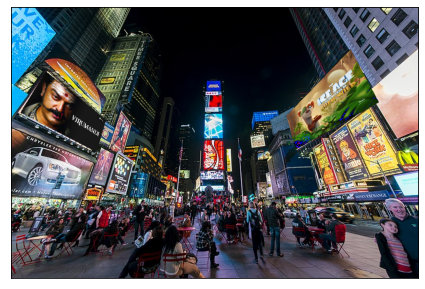
\includegraphics[width=.95\columnwidth]{q2_2}
            \caption{Overlayed Image}
            \label{rst_1}
        \end{minipage}
    \end{center}
\end{figure}


\section{SIFT Feature Matching}
Sift descriptor divides the image into $4\times 4$ sub-patches. Histograms are developed based on the data extracted from each patch using the orientation calculated and normalized to eight discrete levels. These are concatenated to form a feature vector of each feature. Through filtering and matching these feature vectors SIFT achieves robust matchings between points regardless of the variations. Top matches extracted between \textit{im1.ppm} and \textit{im5.ppm} of the Graffiti  images using SIFT is as follows:
\begin{figure}[h]
    \begin{center}
        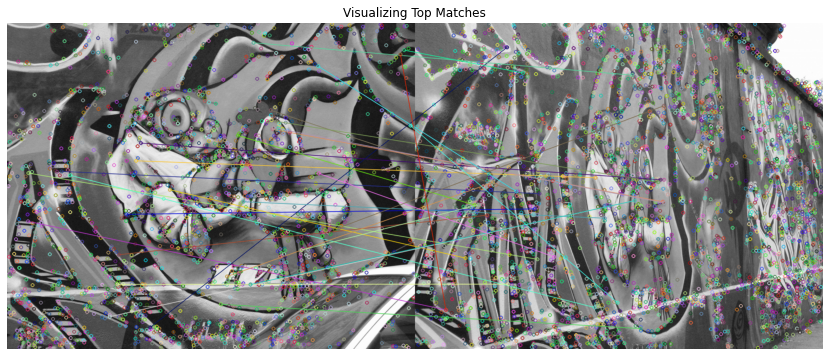
\includegraphics[width=.75\textwidth]{sift}
    \end{center}
\end{figure}
\section{The RANSAC}
\vspace*{-.2cm}
Fitting a model in a set of noisy features leads to unacceptable models. In such cases, it is critical to differentiate between inliers and outliers. RANSAC is a strategy that could be adapted to find the best model fit even in noisy scenarios. The key idea of the approach is to let each point vote for all the models that are compatible with it. The model with the most votes is chosen as the best fit.
\vspace*{-.2cm}
\subsection*{Algorithm}
\vspace*{-.2cm}
\begin{enumerate}
    \item Draw minimum number of points required to fit a model uniformly at random and fit model to the points.
    \item Find the count of inliers to the model (points whose distance or residual w.r.t model is less than threshold)
    \item If there are enough inliers, accept the model.
    \item Perform this until the maximum iteration count required is reached.
    \item Find the best model from the accepted models and refit using all the model points.
\end{enumerate}
\vspace*{-.4cm}
\subsection*{Python Implementation}
\vspace*{-.2cm}
\inputpython{sections/code_listing.py}{64}{88}
\vspace*{-.2cm}





\section*{Scenario-I : Fitting Circle}
\vspace*{-.2cm}
The following figures(\ref{circ},\ref{line}) illustrate two circular models approximated for the points depicted by dots. With proper tuning of the threshold, parameters of first model(\ref{circ},R=9.856 \& O$\equiv$[0.123,-0.156]) stays closer to the parameters of the circle used to create half of these noisy points(R=10 \& O$\equiv$[0,0]). The second model(\ref{line}) seems to depict the nature of noisy line used to create half the data points.
\begin{figure}[h]
    \begin{minipage}{.48\textwidth}
        \begin{center}
            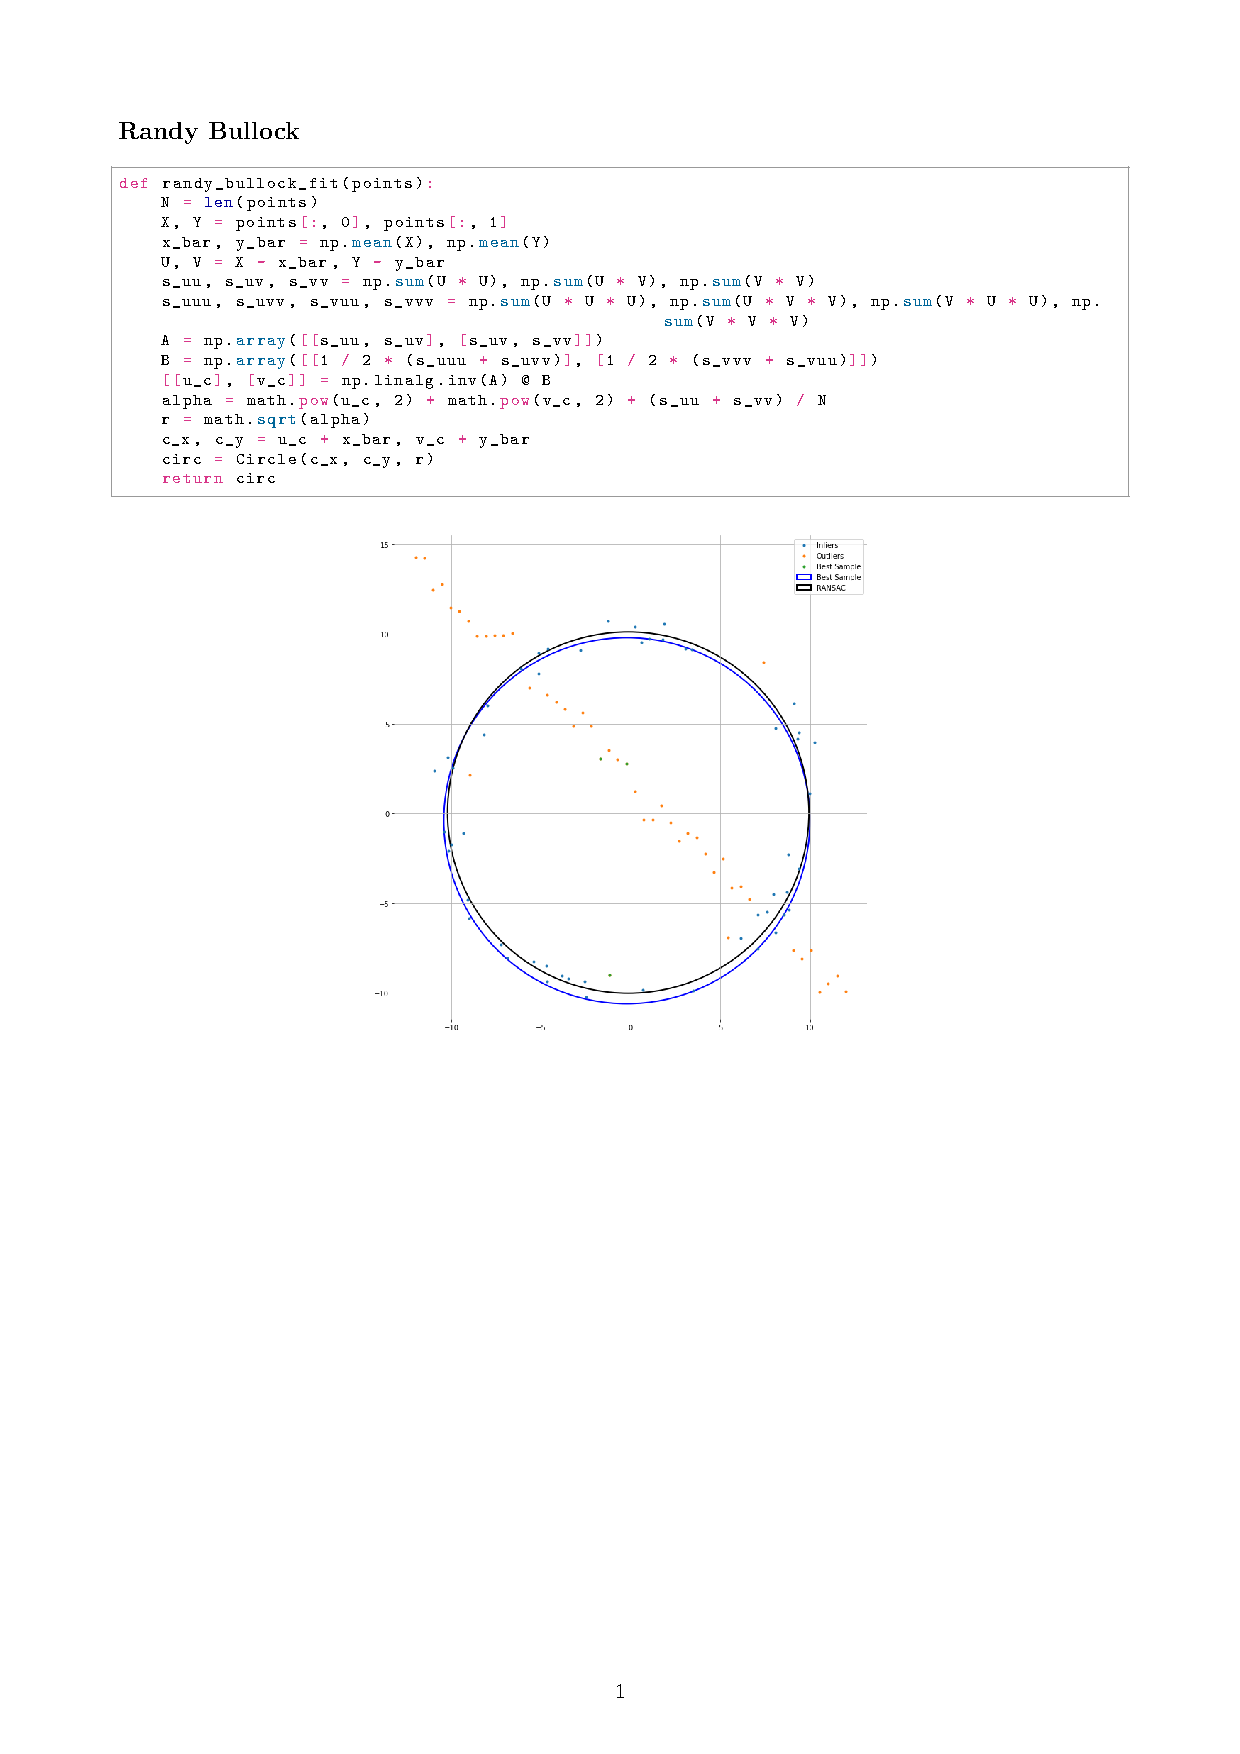
\includegraphics[width=.75\columnwidth]{circle}
            \caption{Model I}
            \label{circ}
        \end{center}
    \end{minipage}
    \begin{minipage}{.48\textwidth}
        \begin{center}
            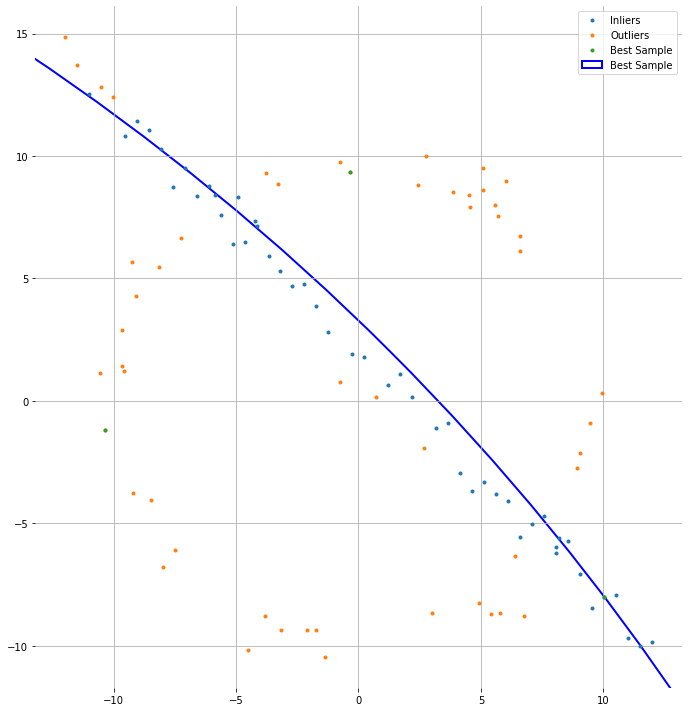
\includegraphics[width=.75\columnwidth]{line}
            \caption{Model II}
            \label{line}
        \end{center}
    \end{minipage}
\end{figure}
\newpage
\section*{Scenario-II : Fitting Homography}
The following figures show the transformation of the Graffiti \textit{im1.ppm} onto \textit{im5.ppm} using the provided homography. Consider the area enclosed using the green-colored bounding box. The transition between two images is almost indistinct and it will be completely seamless if the intenseness of the pixels around the transitions are accurately matched.
\begin{figure}[h]
    \begin{center}
        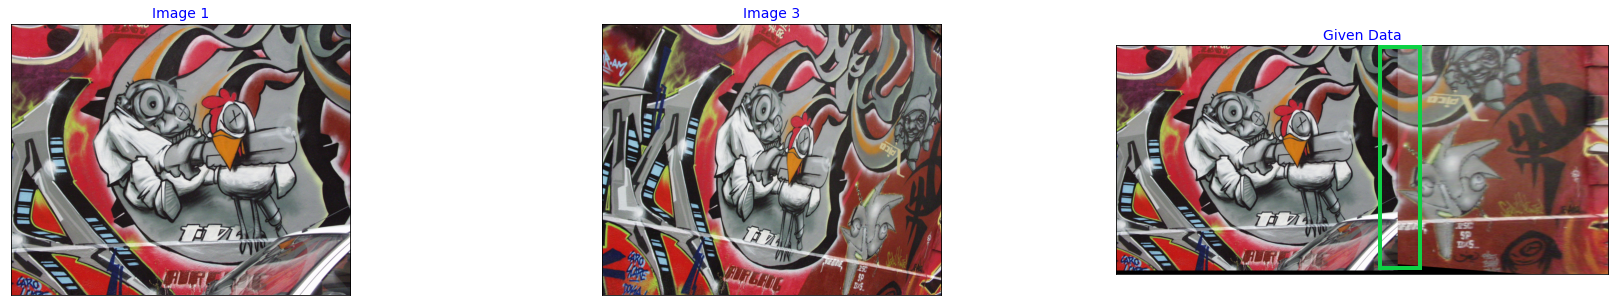
\includegraphics[width=\columnwidth]{q3_1}
    \end{center}
\end{figure}
\\
The following illustration shows the same stitching using the homography extracted from a RANSAC implementation. Firstly the matching features between two images are extracted using the SIFT feature. Then these features are matched using a RANSAC execution with proper thresholding to achieve the transformation homography.
\begin{figure}[h]
    \begin{center}
        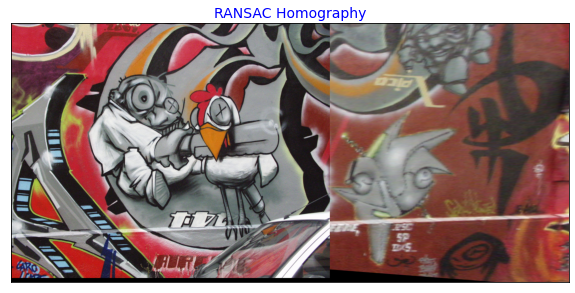
\includegraphics[width=.75\columnwidth]{q3_2}
    \end{center}
\end{figure}
\\
Direct matching between the two images doesn't seem to work due to the scarcity of good matching feature count. Hence it is decided to match adjacent figures(img1 \& img2, img2 \& img3....) which are having more than 1000 matches. And deriving the overall transformation by multiplying adjacent ones. Although a slight translation is visible inside the green bounding box the result can be regarded as a tighter extraction for a basic implementation.
$$H_{1\to5}=H_{4\to5}\cdot H_{3\to4}\cdot H_{2\to3}\cdot H_{1\to2}$$
\vspace*{.2cm}
\begin{minipage}{.48\textwidth}
    \begin{equation*}
        H_{given}=\begin{bmatrix}
            0.625 & 0.058 & 222.012 \\
            0.222 & 1.165 & -25.606 \\
            0.001 & 0.000 & 1.000
        \end{bmatrix}
    \end{equation*}

\end{minipage}
\begin{minipage}{.48\textwidth}
    \begin{equation*}
        H_{ransac}=\begin{bmatrix}
            0.594 & 0.023 & 227.644 \\
            0.215 & 1.066 & -8.788  \\
            0.001 & 0.000 & 1.000
        \end{bmatrix}
    \end{equation*}
\end{minipage}
\section*{References}
\begin{enumerate}
    \item \href{https://dtcenter.org/sites/default/files/community-code/met/docs/write-ups/circle_fit.pdf}{Randy Bullock Fit}
    \item \href{https://docs.opencv.org/4.x/}{opencv}
    \item \href{https://sdg002.github.io/ransac-circle/index.html}{An article about implementation of RANSAC for circle fitting.}
    \item \href{https://programmer.group/panoramic-stitching-using-ransac-algorithm.html}{Panoramic stitching using RANSAC algorithm}
    \item \href{https://youtu.be/J1DwQzab6Jg}{Youtube playlist on Image Stitching}
\end{enumerate}
\vspace*{.8cm}
\HRule
\vspace*{-.2cm}
\begin{center}
    Executable code for the assignment can be found \href{https://github.com/sanjith1999/EN2550-Assignments/tree/master/Fitting%20and%20Alignment}{here}
\end{center}
\end{document}
